\section{ SR06US23 }


\subsection{Meta}

    \textbf{Title:}
    A Review of Reinforcement Learning for Natural Language Processing, and Applications in Healthcare

    \begin{table}[H]
        \centering
        \begin{tabular}{|c|c|c|c|c|c|c|c|c|}
            \hline
                \textbf{Rank} & \textbf{Grasp} & \textbf{Grade} & \textbf{Type} & \textbf{Outcome} & \textbf{Domain} & \textbf{COV19} & \textbf{CoI} & \textbf{DB} \\
            \hline
                2 & 85\% & C & A & P & B & Yes & Yes & No \\
            \hline
        \end{tabular}
        \caption{Reference's metadata}
        \label{tab:SR06US23}
    \end{table}

\subsection{Summary}
    Ying Liu et al. \cite{x090}

\subsection{Notes}
    \begin{itemize}
        \item Systematic Review, Meta-Analysis (PRISMA);
        \item Ovid MEDLINE(R), PubMed, Scopus, Web of Science, ACM Digital Library, and IEEE Xplore; 
        \item IBM Watson was a leafing QA;
        \item ROUGE score evaluates summarisation ML tools;
        \item Text simplification is scored by SMOG;
    \end{itemize}


\subsection{Reading}
    \textbf{Abstract:}
    Reinforcement learning plays a significant role in healthcare management. The current study presents the establishing of ML for medical services, use if RL for Natural Language Processing problems, machine-human human-like communication, and ethical concerns in the field.
    
    \textbf{Objectives:}
    Assess the impact of modern technologies on healthcare.
    
    \textbf{Page 1-2 (Introduction):}
    The growth of the population and the introduction ChatGPT in the world motivated this literature review. The rest of the section is a speed run through the AI history and structure of this article.
    \begin{figure}[H]
        \centering
        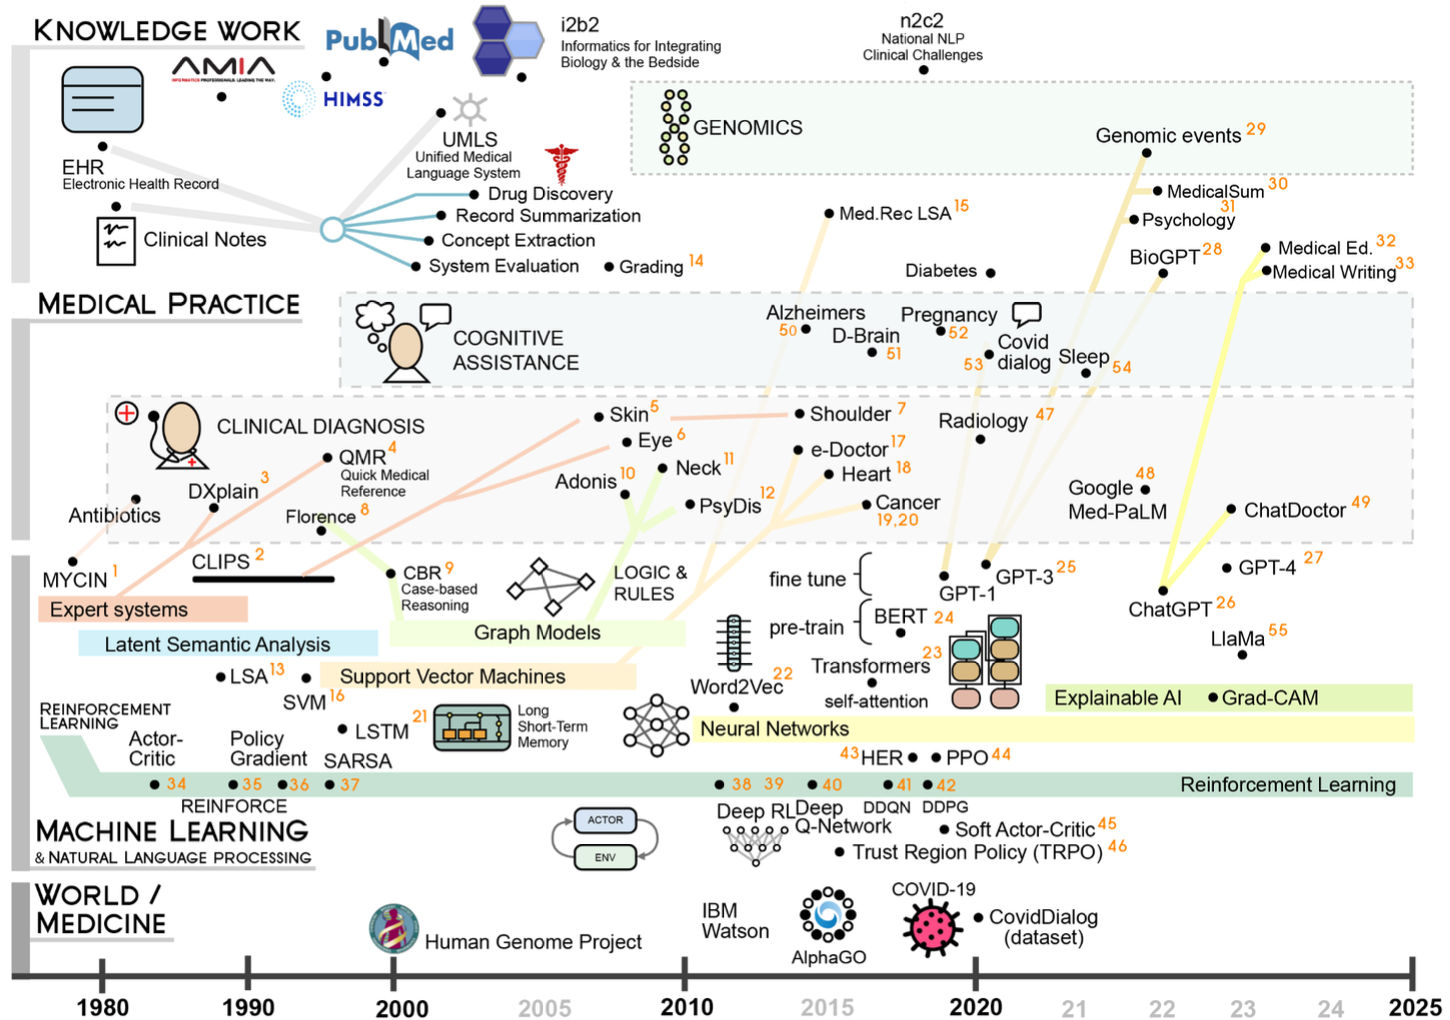
\includegraphics[width=1\textwidth]{figures/0022_SR06US23/fig1.png}
        \caption{AI roudmap from 1980 to now, from \cite{x090}.}
        \label{fig1:0022_SR06US23}
    \end{figure}
    
    \textbf{Page 3-4 (Method):}
    \begin{figure}[H]
        \centering
        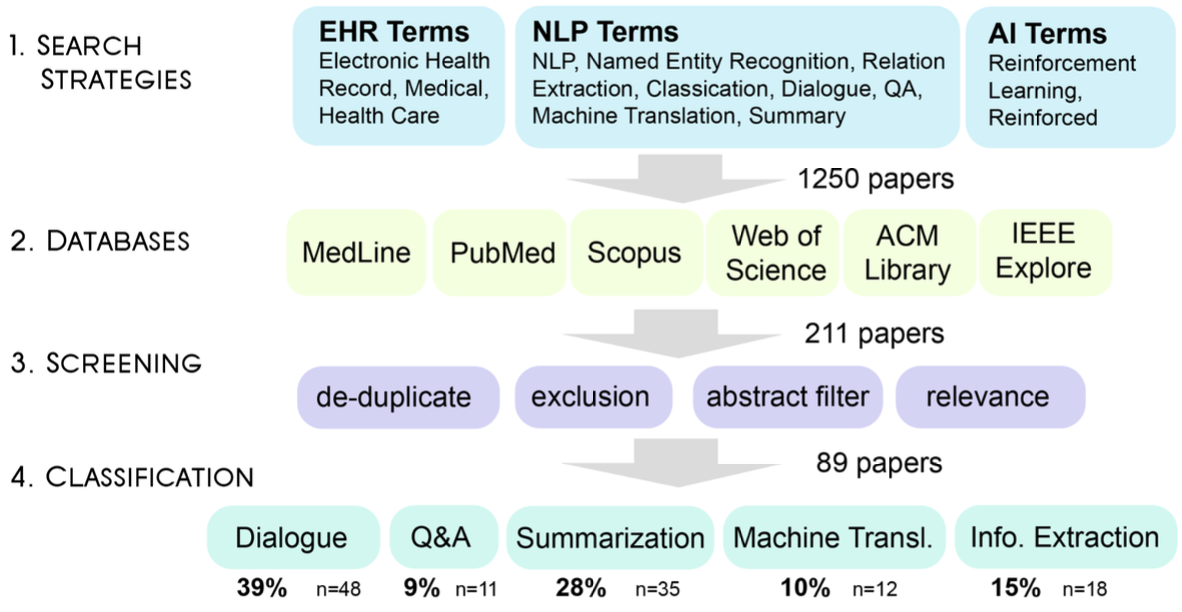
\includegraphics[width=1\textwidth]{figures/0022_SR06US23/fig2.png}
        \caption{Literature search strategy in \cite{x090}.}
        \label{fig2:0022_SR06US23}
    \end{figure}
    \begin{figure}[H]
        \centering
        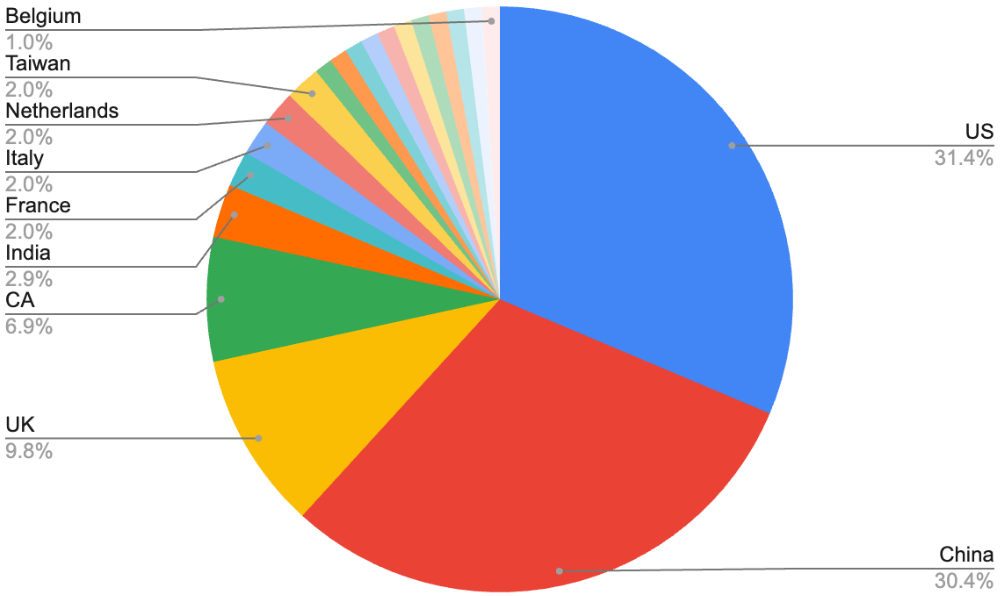
\includegraphics[width=1\textwidth]{figures/0022_SR06US23/fig3.png}
        \caption{Authors' nationalities in \cite{x090}.}
        \label{fig3:0022_SR06US23}
    \end{figure}
    
    \textbf{Page 4-12 (Applied RL and NLP Techniques in Healthcare):}
    \underline{Applied RL} = state + action + reward. There are on-policy and off-policy (Q-learning) methods. RL also classified as model-based and model-free. The next subsection is about dialogues systems, their examples, and summaries. Dialogues sistems (1) require a lot of data to traine and fine tune, (2) they improve healthcare significantly, (3) data safety conserns, (4) require evaluation by human. Then the history and the examples of QA platforms are presented. Machine translation models help to overgo the language barriers for non-English speakers. However, there is still a risk of hurm to patient because of inaccurate translation. Biometric domain has an obsticles such as jargones and technical terminology.
    \begin{figure}[H]
        \centering
        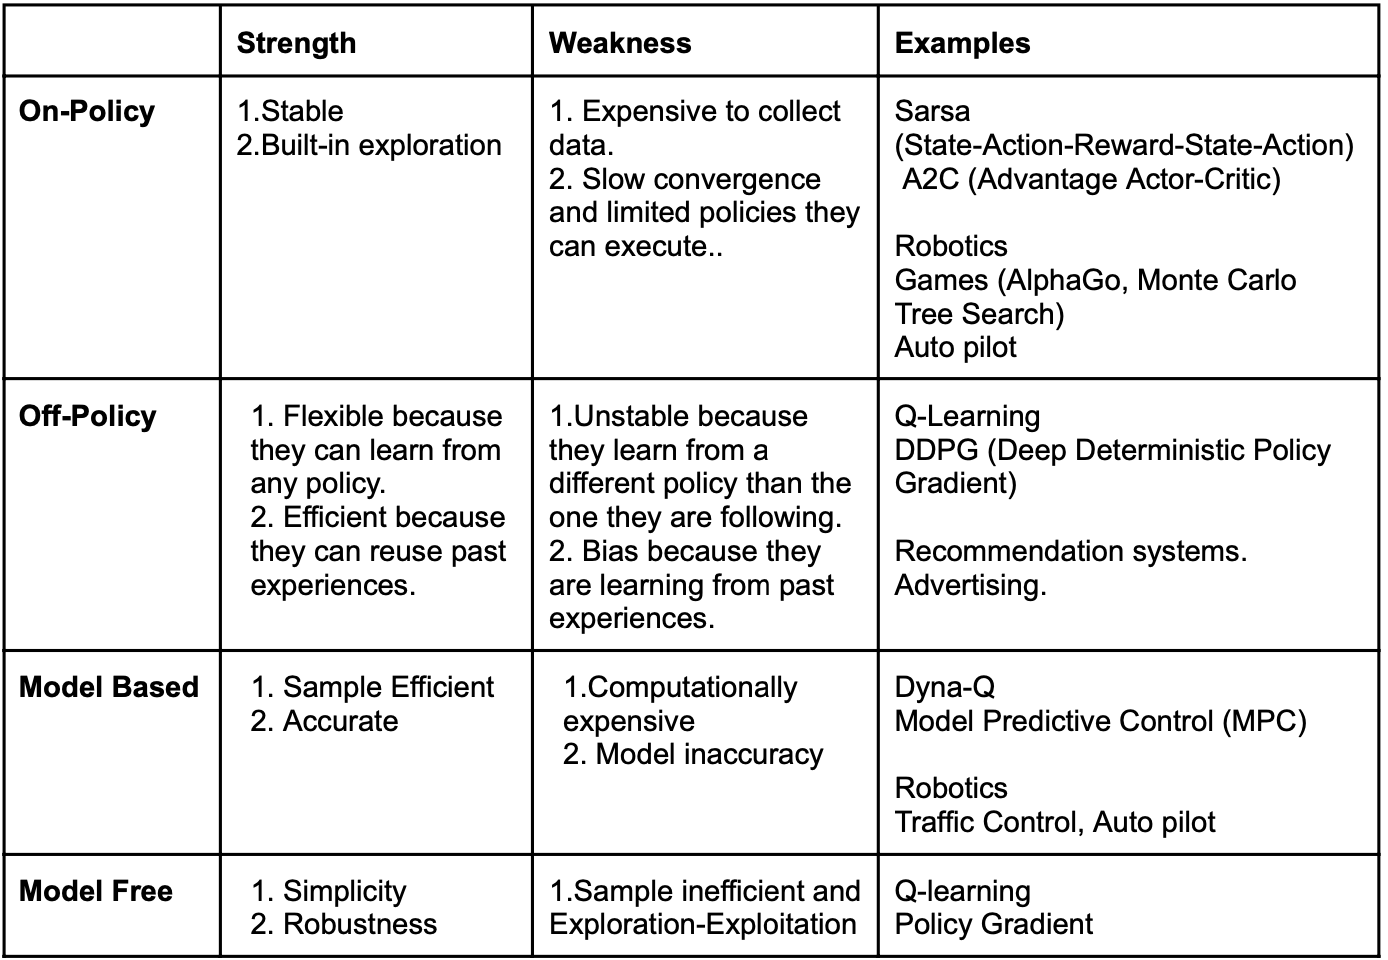
\includegraphics[width=1\textwidth]{figures/0022_SR06US23/fig4.png}
        \caption{Comparison table for RL models from \cite{x090}.}
        \label{fig4:0022_SR06US23}
    \end{figure}
    \begin{figure}[H]
        \centering
        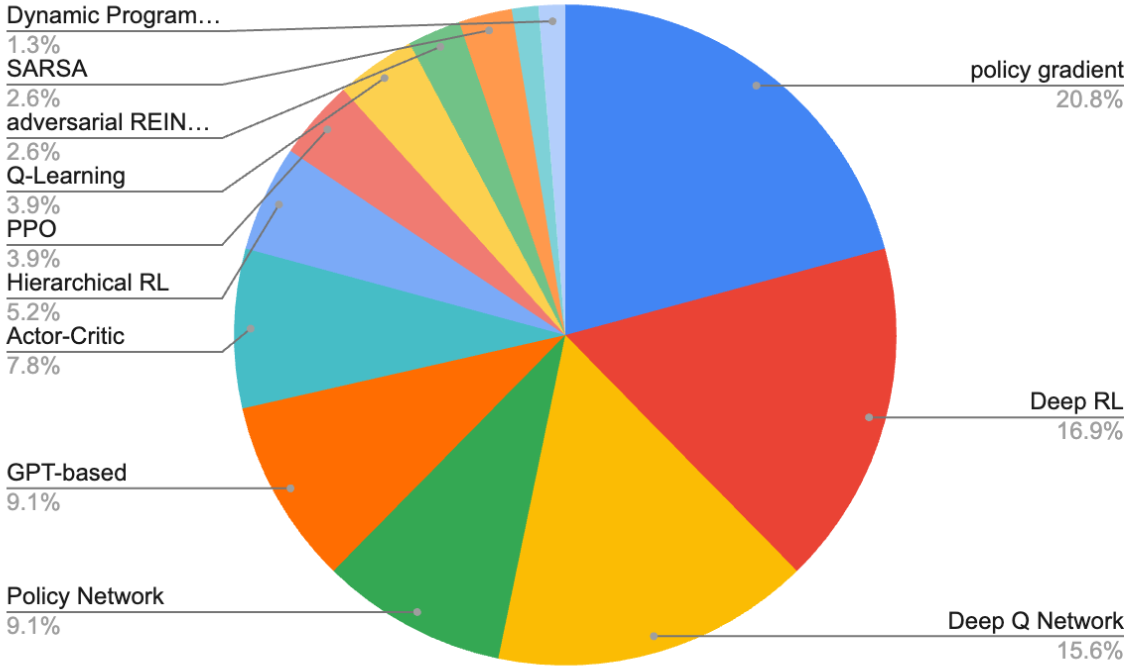
\includegraphics[width=1\textwidth]{figures/0022_SR06US23/fig5.png}
        \caption{Trends of RL models from \cite{x090}.}
        \label{fig5:0022_SR06US23}
    \end{figure}

    \textbf{Page 12 (Discussion):}
    ChatGPT is a suitable NLP for integrating it in RL in healthcare. Nevertheless the challenges related to data security and required data volumes are still need to be concered. 
    \begin{figure}[H]
        \centering
        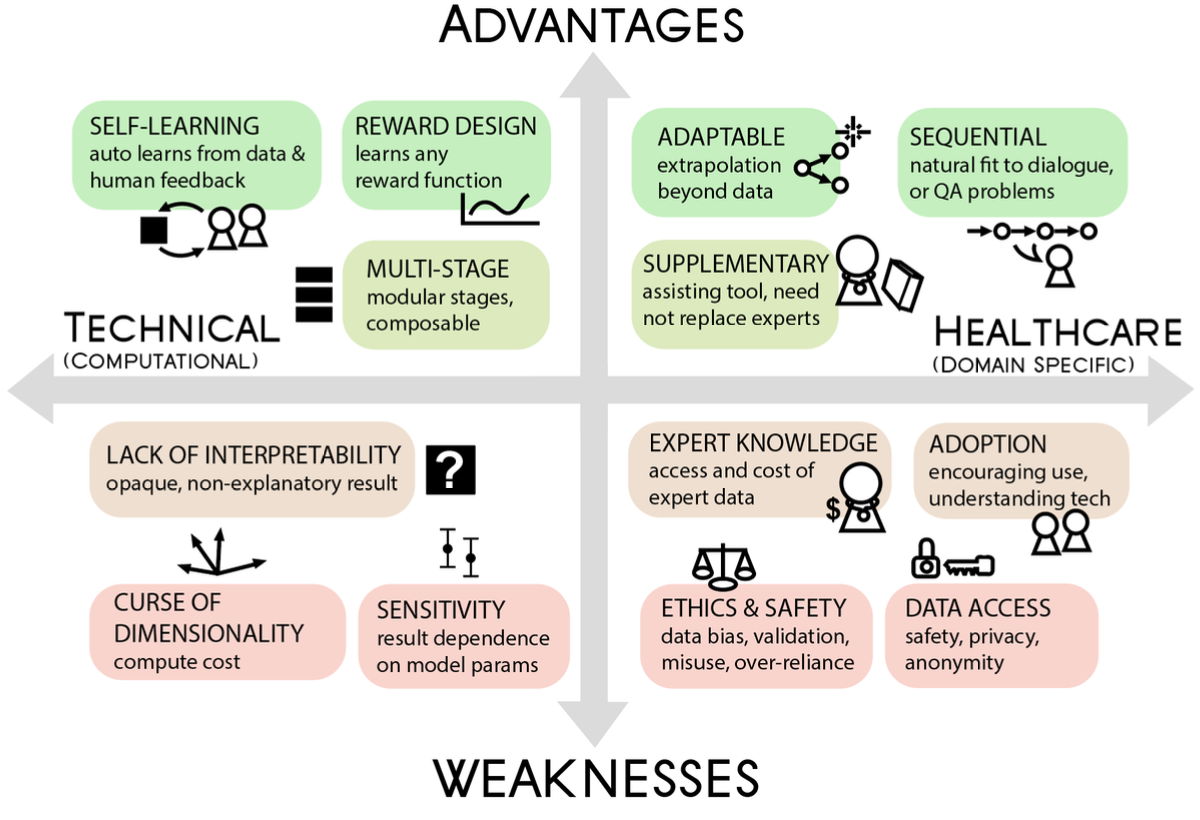
\includegraphics[width=1\textwidth]{figures/0022_SR06US23/fig6.png}
        \caption{RL proc and cons for healthcare domain from \cite{x090}.}
        \label{fig6:0022_SR06US23}
    \end{figure}